\subsection{Krypton Measurement with Delayed Coincidence Analysis}
\label{secDelayedCoincidenceKr85}

Natural krypton contains 10$^{-11}$ of radioactive $^{85}$Kr~\cite{Kr85abundance_1, Kr85abundance_2}, which undergoes $\beta^{-}$ decay with a half-life of 10.756~years and an endpoint energy of 687.1~keV. With 99.563\% branching ratio it emits only an electron, but with 0.434\% probability it decays via the $^{85\mathrm{m}}$Rb metastable state, which de-excites with a $\gamma$-ray emission (see Fig.~\ref{figKr85coincidence}). This delayed $\beta$-$\gamma$ coincidence is used to measure the concentration of krypton in the liquid xenon target, similar to the $\beta$-$\alpha$ coincidence method used to infer the $^{222}$Rn concentration, as described in Section~\ref{secDelayedCoincidenceRn222}. 

%\begin{equation}
%\nonumber
%\text{Kr85(\beta, 173.4~keV) \rightarrow Rb85m(\gamma, 514~keV, 1.46~\mu s) \rightarrow Rb85
%\end{equation}

\begin{figure}[!h]
\centering
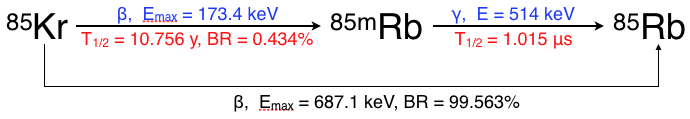
\includegraphics[width=0.55\linewidth]{plots/Kr85/Kr85coincidence1.png}
\caption{Decay channel of $^{85}$Kr used to measure krypton concentration with a delayed coincidence method}
\label{figKr85coincidence}
\end{figure}

\begin{floatingfigure}[l]{0.39\textwidth}
%\begin{figure}[!h]
\centering
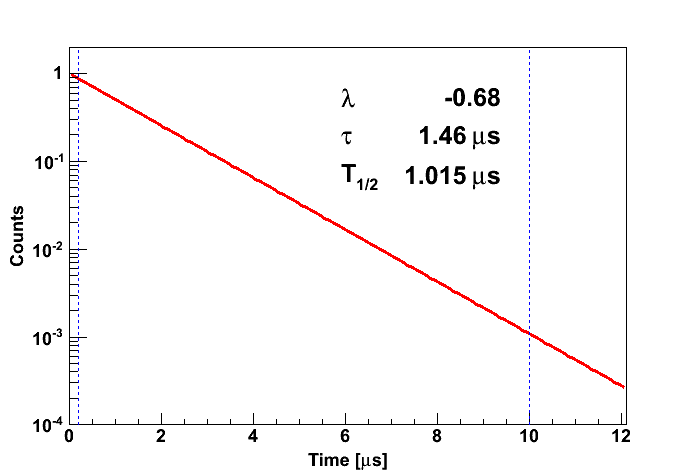
\includegraphics[width=0.39\linewidth]{plots/Kr85/DelayTime_Kr85.png}
%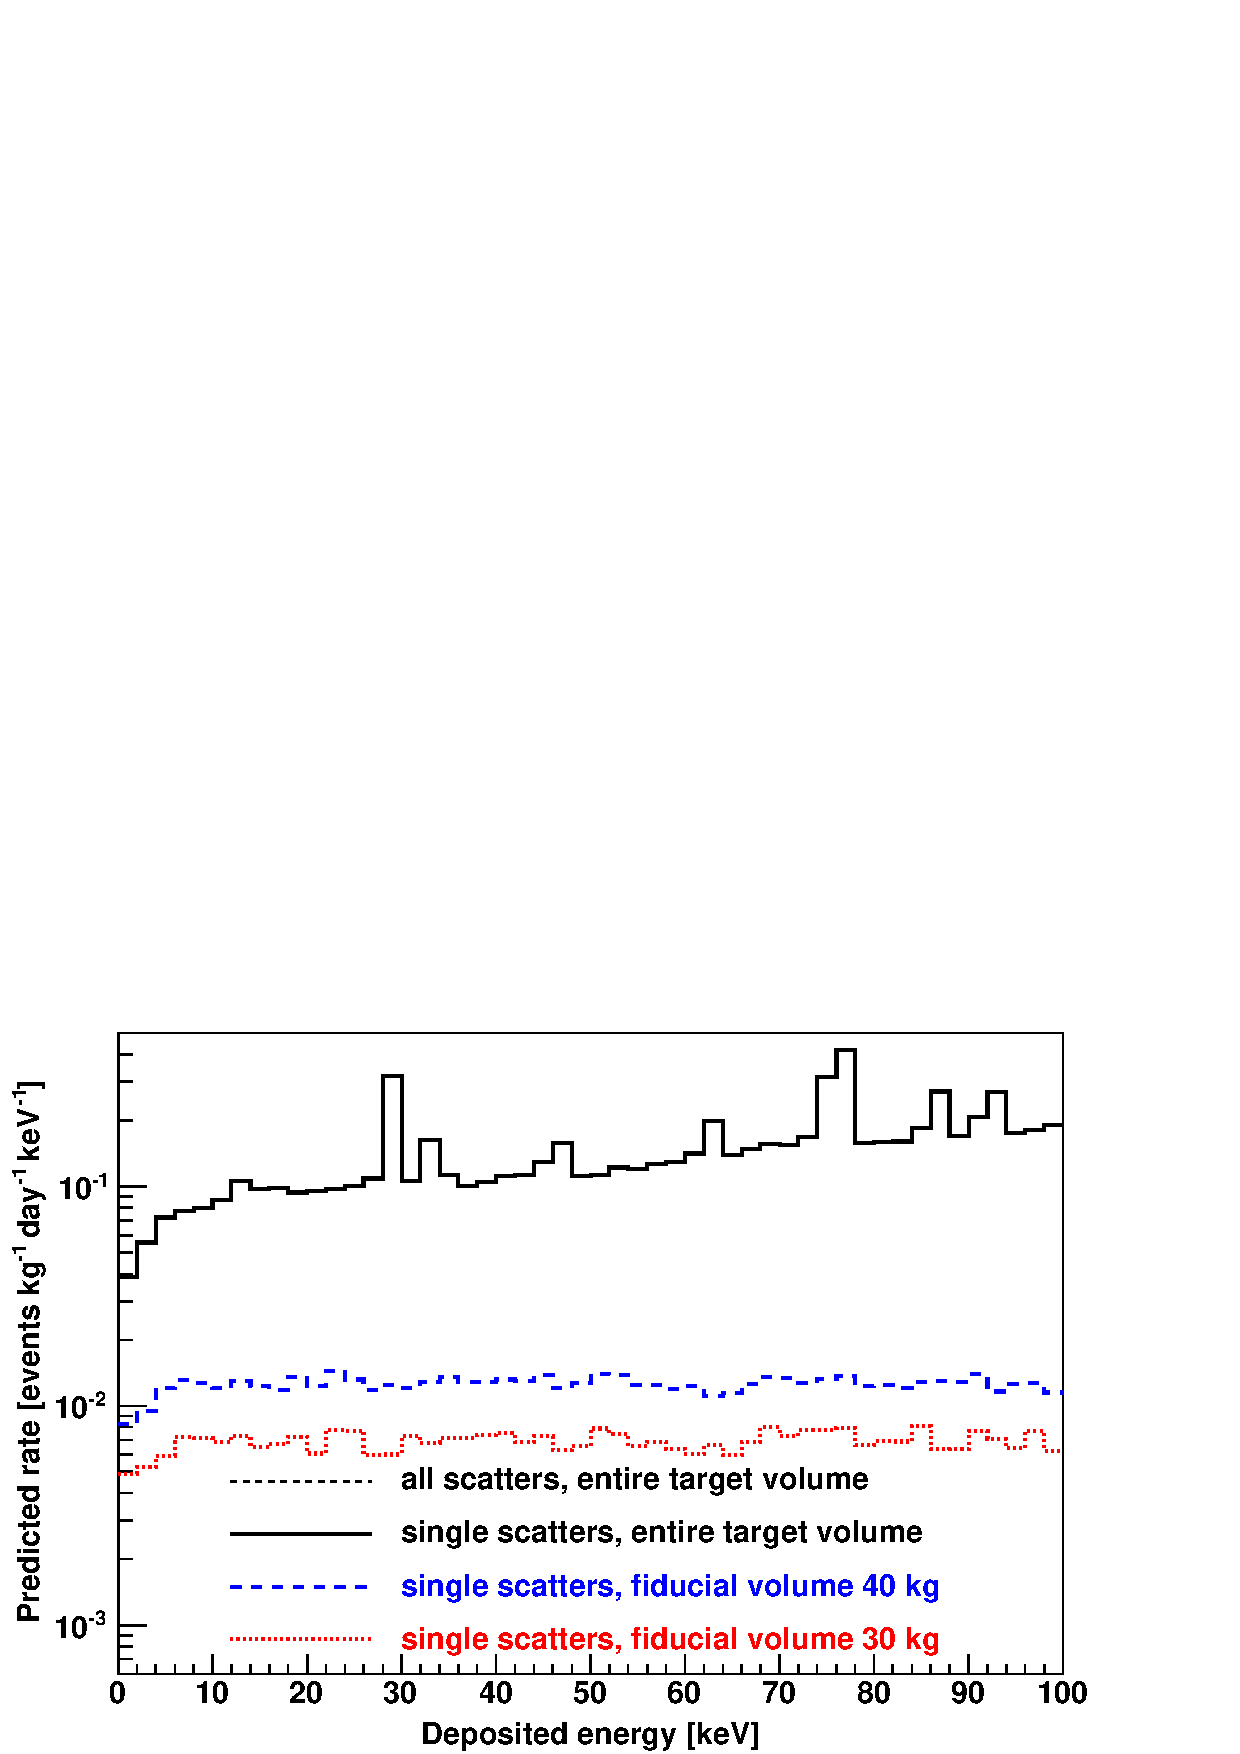
\includegraphics[height=0.7\linewidth]{plots/SpectraWS_withFV40andFV30_50bins_dot.png}
\caption[Expected delay time between coincident $\beta$ and $\gamma$ from $^{85}$Kr decay]{Expected delay time between coincident $\beta$ and $\gamma$ from $^{85}$Kr}% decay.} %The dashed blue lines indicate the time window defined for the analysis.}
\label{figKrDelayTime}
%\end{figure}
\end{floatingfigure}

The detection efficiency has been calculated using equation (\ref{eqDetectionEfficiency}).
The time window to search for coincident events is defined as $t_{2}$ = 10~$\mu$s. Since the peak finder can resolve two S1 peaks which are separated by at least 300~ns, this defines the lower bound for the search window($t_{1}$). The expected distribution of the delay time between $\beta$ and $\gamma$ is shown in Fig.~\ref{figKrDelayTime}, with the blue lines indicating the search window. The acceptance of the timing cut, shown in the dashed blue lines is 81.3\%. \par
The energy cut for $\gamma$-interaction has been designed as $\pm$2$\sigma$ around the central value of 514~keV, taking into account the S1 resolution, the light yield at this energy (1.6 PE/keV), and the variation of S1 LCE in the TPC (see Section~\ref{secLCEs1}). The energy cut for  the $\beta$ has been chosen to include the widest possible range without an overlap with the region defied for the $\gamma$. The combined acceptance of these energy cuts is 90\%, which gives a total detection efficiency of 73.2\%. 
Waveforms of $^{85}$Kr candidate events tagged with the delayed coincidence method are shown in Fig.~\ref{figKr85WF}.  The S1 spectra of the interactions are shown in Fig.~\ref{figDCrun08_1}.  The measured distribution of the delay time between the $\beta$ and $\gamma$ interactions is shown in Fig.~\ref{figDCrun08_2}. The measured half-life of $^{85\mathrm{m}}$Rb and the energy spectra are in a good agreement with the expectation. 

\begin{figure}[!h]
\centering
\subfigure[]{
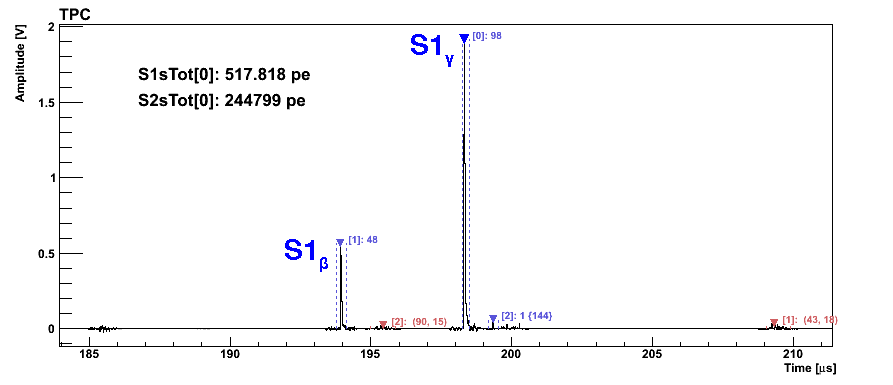
\includegraphics[width=0.475\linewidth]{plots/Kr85/Kr85WF1_withLabels.png}
\label{figKr85WF_1}}
\subfigure[]{
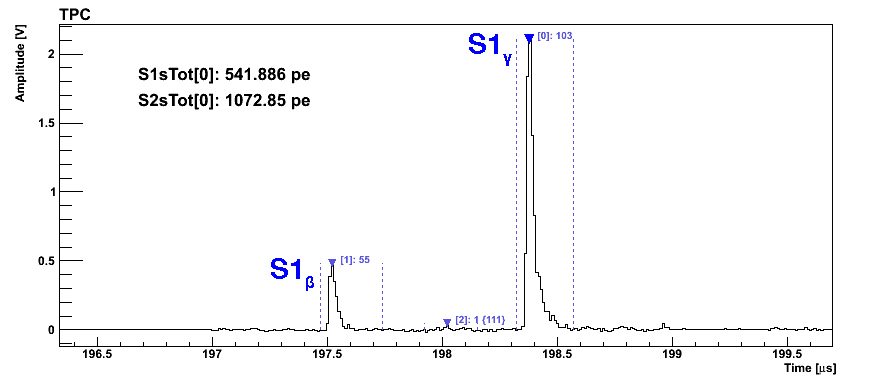
\includegraphics[width=0.475\linewidth]{plots/Kr85/Kr85WF3_withLabels.png}
\label{figKr85WF_2}}
\caption{Waveforms of $^{85}$Kr candidate events tagged with the $\beta$-$\gamma$ delayed coincidence method.}
\label{figKr85WF}
\end{figure}


\begin{figure}[!h]
\centering
\subfigure[]{
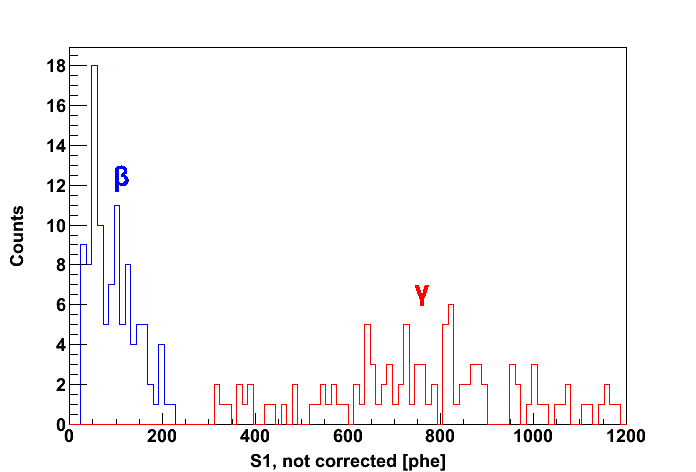
\includegraphics[width=0.475\linewidth]{plots/Kr85/S1_run08_withLabels.png}
\label{figDCrun08_1}}
\subfigure[]{
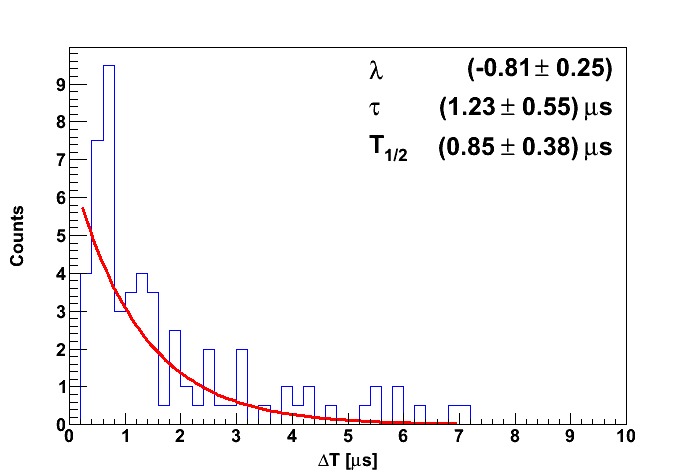
\includegraphics[width=0.475\linewidth]{plots/Kr85/dt_run08_withFit.png}
\label{figDCrun08_2}}
\caption[The S1 spectra of the $\beta$ and $\gamma$ interactions tagged in the data of the first science run and delay time distribution]{The S1 spectra (a) of the $\beta$ and $\gamma$ interactions (blue and red, respectively) tagged in the data of the first science run and delay time distribution (b). Within the statistical error of the measurement, the half-life of (0.85$\pm$0.38)~$\mu$s is in agreement with the expectation of 1.015~$\mu$s.}
\label{figDCrun08}
\end{figure}

Due to the low rate, the probability function for the number of measured events follows a Poisson distribution and is shown as an example for run08 in Fig.~\ref{figPDF_1}. The confidence regions have been computed with the graphical maximum likelihood method~\cite{StatisticsCowan},  illustrated in Fig.~\ref{figPDF_2},  by finding the values of $N$ at which the log-likelihood function logL($N$) decreases by 2.71/2 for 90\% , and by 3.84/2 for 95\% confidence level from its maximum value logL$_{\mathrm{max}}$.

%From the observed number of events, the decay rate (events s-1 kg-1) of 85Kr (in units [Bq/kg]) is calculated:
The activity of $^{85}$Kr is calculated from the measured number of $\beta$-$\gamma$ coincident events as:
%R1 = N ? time-1 ? massLXe-1
\begin{equation}
A\ \text{[Bq/kg]} = \frac{N}{\Delta t \cdot m_{\mathrm{LXe}} \cdot \xi \cdot \eta},
\end{equation}
where $N$ - number of observed coincident events, $\Delta t$ - live time of the analyzed data, $m_{\mathrm{LXe}}$ - mass of the liquid xenon (62~kg in this analysis), $\xi$ - branching ratio of the tagged decay channel (0.434\%), $\eta$ - detection efficiency (73.2\%).

\begin{figure}[!t]
\centering
\subfigure[]{
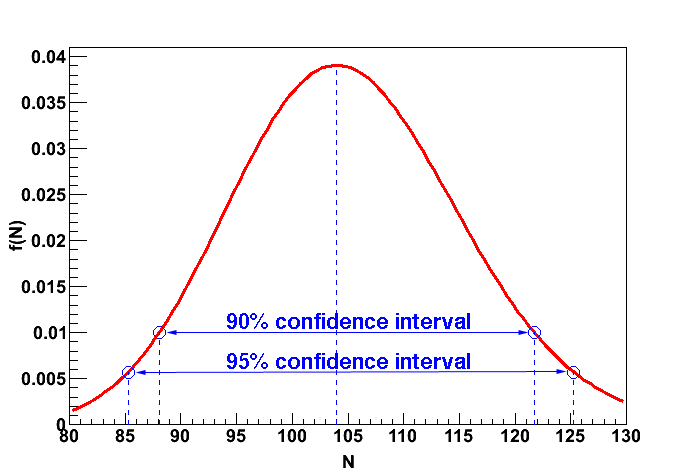
\includegraphics[width=0.475\linewidth]{plots/Kr85/PDF_run08_withLabels.png}
\label{figPDF_1}}
\subfigure[]{
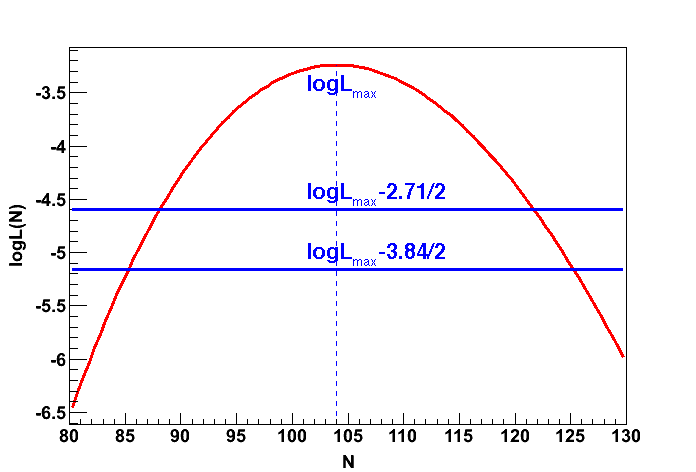
\includegraphics[width=0.475\linewidth]{plots/Kr85/LogL_run08_withLabels.png}
\label{figPDF_2}}
\caption[Probability function and log-likelihood for $^{85}$Kr candidate events observed in the first science run data]{Probability function (a) and log-likelihood (b) for $^{85}$Kr candidate events observed in the first science run data. The 90\% and 95\% confidence regions have been computed with the graphical maximum likelihood method.}
\label{figPDF}
\end{figure}

The measured activity of $^{85}$Kr is converted to the concentration of natural krypton:
\begin{equation}
C\ \text{[Kr/Xe mol/mol]} = \frac{A \cdot \tau \cdot M_{\mathrm{Kr}}}{N_{A} \cdot M_{\mathrm{Xe}} \cdot k},
\end{equation}
where $A$ - activity of $^{85}$Kr in [Bq/kg], $\tau$ - mean lifetime of $^{85}$Kr, $N_{A}$ - Avogadro number, M$_{\mathrm{Kr}}$ and M$_{\mathrm{Xe}}$ - atomic weights of krypton and xenon, respectively, $k$ - abundance of $^{85}$Kr in natural krypton.

%Finally, the concentration of natural krypton in xenon, is calculated:
%\begin{equation}
%C_{1}\ [Kr/Xe mol/mol] = \frac{C}{Ab}, 
%\end{equation}
%where C1 - concentration of 85Kr (Kr/Kr [mol/mol]), AB85 - abundance of 85Kr in natKr (10-11), BR85 - branching ratio of the tagged decay channel (0.434\%), Kr/Xe - ratio of atomic mass of Kr and Xe, %? - detection efficiency (0.786 for runs 07 and 10, and 0.702 for run08).

The concentration of natural krypton measured with the delayed coincidence method is presented in Table~\ref{tabKrypton}. Due to the low branching ratio of the tagged decay channel, the method is limited by statistics. Better sensitivity can be achieved, for example, with mass spectrometry~\cite{KryptonMS} or atomic trap trace analysis methods~\cite{KryptonATTA}. Prior to the start of the data acquisition period of the first science run, additional krypton has been introduced by an air leak during maintenance work on the gas recirculation. Before the second science run, the xenon has been purified by cryogenic distillation, which reduced the concentration of krypton to the level measured in the commissioning run in Fall 2009.

\begin{table}[!h]
\centering
\caption{Krypton concentration measured with delayed coincidence analysis.}
\label{tabKrypton}
%\vspace{0.2cm}
\begin{tabular}{>{\footnotesize}l |>{\footnotesize} c |>{\footnotesize} c |>{\footnotesize} c |>{\footnotesize} c}
%\begin{tabular}{l | c | c | c | c}
\hline
									& Livetime [days]	& Events	& \multicolumn{2}{>{\footnotesize}c}{$^{\mathrm{nat}}$Kr conc. [ppt mol/mol]} \\
									&				&		& 90\% C.L.			& 95\% C.L. \\
\hline
%\vspace{0.1cm}
%run07, all data						& 40.402			& 19		&  297$^{+127}_{-98}$	& 297 +154 -114 \\
run07, commissioning run \cite{xe100-run07}	& 11.17			& 3		&  88$^{+112}_{-59}$	& 88$^{+141}_{-66}$  \\
%\vspace{0.1cm}
%run07, after Dec.~1 					&				& 16		&  532$^{+250}_{-190}$	&  \\
run08, first science run \cite{xe100-run08}	& 100.915			& 104	&  650$^{+111}_{-94}$	& 650$^{+133}_{-117}$  \\
%\vspace{0.1cm}
run10, second science run 				& 32.123			& 7		&  138$^{+104}_{-69}$	& 138$^{+128}_{-78}$  \\
\hline
\end{tabular}
\end{table}


%90\% confidence [ppt mol/mol]
%95\% confidence [ppt mol/mol]
%run 07, entire run 	
%297 +127 -98
%297 +154 -114
%run 07, before Dec.1	
%88 +112 -59
%88 +141 -66
%run 07, after Dec.1 	
%532 +250 -190
%532 +250 -220
%run 08 	
%650 +111 -94
%650 +133 -117
%run 10 	
%138 +104 -69	
%138 +128 -78



